\documentclass[../main]{subfiles}
\begin{document}

\section{Konventionen und Notation}

\subsection*{Beschriftung}

\begin{center}\textbf{Zahlen und Tensoren}\end{center}
\begin{tabular}{cl}
  $a$ & ein Skalar (Zahl) \\
  $\vec{a}$ & ein Vektor \\
  $\mat{A}$ & eine Matrix \\
  $\mat{A}_{n \times m}$ & Matrix mit $n$ Zeilen und $m$ Spalten \\
  $\ten{A}$ & ein Tensor \\
  $\mathfrak{A,B,C,D,E,\cdots}$ & a \\
  $\mathfrak{a,b,c,d,e,f,g,\cdots}$ & a \\


\end{tabular}

\begin{center}\textbf{Mengen}\end{center}
\begin{tabular}{cl}
  $(a,b)$ & ein geordnetes Paar (2-Tupel) der Elemente $a$ und $b$ \\
  $\set{A}$ & eine Menge \\
  $\set{R}$ & die Menge aller Reeller Zahlen \\
  $\set{Z}$ & die Menge aller ganzer Zahlen \\
  $\set{N}$ & die Menge aller natuerlicher Zahlen \\
  $\set{E}$ & die Menge aller gerader (engl.: even) Zahlen \\
  $\set{O}$ & die Menge aller ungerader (engl.: odd) Zahlen \\
  $\{a,b\}$ & die Menge, welche aus Elementen $a$ und $b$ besteht \\
  $\{1,\ldots,n\}$ & Menge aller ganzen Zahlen von 1 bis $n$ \\

\end{tabular}

\begin{center}\textbf{Indexierung}\end{center}
\begin{tabular}{cl}
  $\vecelem{a}_i$ & $i$-te Vektorkomponente mit Startindex 1 \\
  $\mat{A}_{n \times m}$ & Matrix mit $n$ Zeilen und $m$ Spalten \\
  $(\mat{A})_{i,j} = $ & Matrixelement in der $i$-ten Zeile und der $j$-ten Spalte \\
  $\matelem{A}_{i,j}$ & Matrixelement in der $i$-ten Zeile und der $j$-ten Spalte \\
  $\mat{A}_{i,:}$ & Zeile $i$ der Matrix $\mat{A}$ \\
  $\mat{A}_{:,i}$ & Spalte $i$ der Matrix $\mat{A}$\ \\

\end{tabular}

\begin{center}\textbf{Lineare Algebra Operationen}\end{center}
\begin{tabular}{cl}
  $\trans{\mat{A}}$ & das Transponierte einer Matrix $\mat{A}$ \\
  $\mat{A} \odot \mat{B}$ & Elementeweises (Hadamard) Produkt \\

\end{tabular}

\begin{center}\textbf{Infinitesimalrechnung/Differentialrechnung}\end{center}
\begin{tabular}{cl}
  $\displaystyle\deriv{y}{x}$ & Ableitung von $y$ bezueglich $x$ \\[2ex]
  $\displaystyle\partderiv{y}{x}$ & Partielle Ableitung von $y$ bezueglich $x$ \\[2ex]
  $\nabla y$ & Gradient von $y$\\
  $\nabla_{\vec{x}}y$ & Gradient von $y$ bezueglich $\vec{x}$ (Vektor) \\

\end{tabular}

\begin{center}\textbf{Funktionen}\end{center}
\begin{tabular}{cl}
  $f: \set{A} \to \set{B}$ & Funktion $f$ mit Definitionsmenge $\set{A}$ und Zielmenge $\set{B}$ \\
  $f(x)$ & Funktion $f$ mit Argument $x$ (Skalar) \\
  $f(\vec{v})$ & Funktion $f$ mit Argument $\vec{v}$ (Vektor) \\
  $f[\vec{v}]$ & Vektorisierte Funktion $f$ mit Argument $\vec{v}$ (Vektor) \\
  $\mathcal{A}$ & ein Funktionenraum \\

\end{tabular}

\begin{center}\textbf{Machine Learning}\end{center}
\begin{tabular}{cl}

\end{tabular}


\pagebreak
\section{Machinelles Lernen - Theorie}

Der Themenbereich des \keyword{Machinellen Lernens} beschäftigt sich mit Algorithmen und mathematischen Modellen, welche von selber lernen, Probleme zu loesen.
Hierzu werden keine expliziten Instruktionen fest einprogrammiert (engl.:\ hard coding), sondern das Modell wird trainiert und optimiert sich von selbst.
Dabei wird das Modell mit Trainingsdaten befuettert, mithilfe dessen eine Korrelation zwischen den Inputdaten und den Outputdaten erlernt werden soll.
Der Zusammenhang der Daten wird von den Modellen verallgemeinert und das Modell kann dann Vorhersagen fuer neue Daten machen.

\subsection{Allgemeine Begriffe}

\subsubsection{Daten}

Um ein Modell zu trainieren braucht man Daten.
Diese Daten kommen in der Form eines \keyword{Trainingsdatensatz} $\set{X}$.
Dabei handelt es sich um eine Menge von \keyword{Trainingssampeln},
welche jeweils aus \keyword{Inputs} und gewuenschten Outputs.
bestehen. Diese gewuenschten Outputs bezeichnet man auch als \keyword{Labels}.
Diese Inputs werden in einem Vektor $\vec{x}=\trans{(x_1,x_2,\ldots,x_n)}$ und
die Labels in einem Vektor
$\vec{\hat{y}}=\trans{(\hat{y}_1,\hat{y_2},\ldots,\hat{y}_m)}$ zusammengefasst.
Die Labels sind zu unterscheiden von den vorhergesagten \keyword{Outputs},
welche der Algorithmus produziert. Auch diese Outputs werden in einem Vektor
$\vec{y}=\trans{(y_1,y_2,\ldots,y_m)}$ zusammengefasst.
Somit ist ein Trainingssample nichts anderes als ein Paar
$(\vec{x}_i,\vec{y}_i)$ eines Inputsvektor $\vec{x}$ und eines Labelvektor
$\vec{\hat{y}}$.
\para{}
Die Inputs bestehen aus gewissen \keyword{Attributen}, welche die
Merkmals\textit{typen} der Daten sind. Die sogennanten \keyword{Features} sind
dann die spezifischen Werte der Attribute eines Samples. Der Algorithmus soll
anhand dieser Attribute seine Vorhersagen machen.
Diese Vorhersagen werden dann mit den Labels abgeglichen und so bewertet.
Anhand der Bewertungen wird dann eine Optimierung des Modells vorgenommen.
Unter korrekten Bedingungen (keine Ueberanpassung) findet kein Auswendiglernen der Trainingsdaten statt,
sondern ein Generalisieren des Zusammenhangs anhand von Mustern und Gesetzmassigkeiten.
\para{}
Um eine endgueltige Bewertung des Modells durchzufuehren, wird ein Testdatensatz
$\set{T}$, welcher nicht Teil des Trainingsdatensatz ist, genutzt um Vorhersagen zu machen.
Dies garantiert, dass kein Auswendiglernen moeglich ist.
\para{}
\par \medskip
BESSERS BEISPIEL -> UM SPAETER KONKRETES MODELL ZU ERKLAEREN
AUTOPREIS SCHAETZEN (OKASSION) ANHAND VON GEFAHRENEN KILOMETERN
Am Beispiel eines Datensatz, welcher fuer Bilderkennung von Hunden und Katzen genutzt wird, werden diese Begriffe verdeutlicht.
Die Inputdaten sind die Fotos von Hunden und Katzen. Deren Attribute sind die moeglichen RGB-Farbenwerte (drei Zahlen, welche von 0 bis 255 reichen) aller Pixel.
Die Features sind die spezifischen RGB-Werte der Pixel fuer die einzelnen Bilder. Die Outputdaten sind die Labels, welche in diesem Fall angeben, ob ein Hund oder eine Katze auf dem Bild gezeigt wird.
Dies wird meistens mit einer One-Hot-Kodierung bzw.\ einem One-Hot-Vektor
gemacht. Jeder Labelart wird eine eigene Vektorkomponente zugewiesen. Falls das
Label aktiv ist, ist die Komponent 1 ansonsten 0. Somit kann Hund als $\vec{l}_H={(1,0)}^T$ reprasentiert werden und Katze als $\vec{l}_K={(0,1)}^T$.

\begin{figure}[h!]
  \centering
  \begin{tikzpicture}[node distance=5cm,auto]

  \end{tikzpicture}

  \caption{das beschriebene Machine Learning Modells}
\end{figure}

\subsubsection{Modelle}
Ein \keyword{Modell} ist eine mathematische Funktion $\mathit{f}\colon \set{R}^n \to \set{R}^m$, welche die Inputs auf die Outputs abbildet $\vec{y}=\mathit{f}(\vec{x})$.
Im Zusammenhang mit Wertevorhersagen spricht man von einem Regressionsmodell.
Das Verhalten dieses Modells wird bestimmt durch seine \keyword{Modellparameter} $\hyperp_1, \hyperp_2,\ldots$.
Das Ziel ist es, die Modellparameter so einzustellen, dass die Vorhersagen $\vec{y}$ besser mit den Labels $\vec{\hat{y}}$ uebereinstimmen.
Dies wird iterativ gemacht, indem immer wieder leichte Anpassungen an den
Parametern vorgenommen werden, bis das Modell die gewuenschten Resultate liefert.
\para{}
Das wohl einfachste Regressionsmodell ist eine Regressionsgerade. Diese ist
angemessen, falls ein einfacher linearen Zusammenhang der Form $y=\hyperp_1x +
\hyperp_0$ zwischen den Features und den Labels besteht.
Nun muessten nur noch $\hyperp_0$ und $\hyperp_1$ bestimmt werden.

Neben den gelernten Parametern, gibt es auch noch sogenannte \keyword{Hyperparameter}.
Diese koennen nicht erlernt werden, sondern muessen manuell vor dem Training gewaehlt werden und koennen den Lernvorgang erheblich beeinflussen.
\para{}
Fuer Machine Learning haben sich gewisse Modelle besonders guet etabliert,
darunter waeren: Support Vector Machines, Evolutionäre Algorithmen, und Künstliche Neuronale Netze.
Diese Arbeit wird sich vorwiegend mit Neuronalen Netzen auseinandersetzen.
\para{}
BEISPIELMODELL GLEICHES WIE VORHIN
% Um den Modellbegriff noch etwas zu festigen wird ein Beispielmodell erlautert:\\
% Das Modell soll Vorhersagen zum Wetter machen. Anhand von Luftfeuchtigkeit und
% Temperatur muss es eine Aussage treffen, ob es gerade regnet oder nicht.

\begin{figure}[h!]
  \centering

  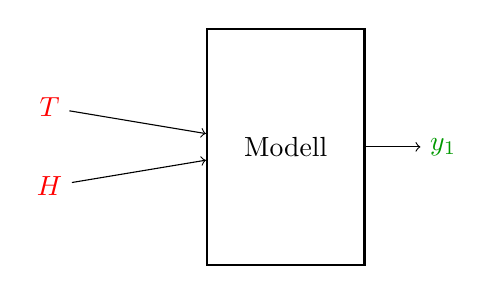
\begin{tikzpicture}
    \path (3,0) node [draw,thick,minimum width=2cm,minimum height=3cm](neuron){Modell};
    \path[red] (0,0.5) node(T){$T$} (0,-0.5) node(H){$H$};
    \path[black!40!green] (5,0) node(y1){$y_1$};
    \draw[->] (T) -- (neuron);
    \draw[->] (H) -- (neuron);
    \draw[->] (neuron) -- (y1);

  \end{tikzpicture}

  \caption{beschriebenes Beispielmodells}
\end{figure}

\subsection{Sonstiges}
\subsubsection{Supervised Learning}
\subsubsection{Unsupervised Learning}
\subsubsection{Overfitting}

\subsection{Training}
\subsubsection{Kostenfunktionen}
Einsicht ist der erste Schritt zur Besserung. Das gilt auch beim Machine Learning, deshalb muss beim Training zuerst die Genauigkeit des Modells bewertet werden.
Dafuer gibt es sogennante \keyword{Kosten-, Verlust- oder Fehlerfunktionen}. Sie sollen ein Mass fuer die Abweichung des Outputs $\vec{y}$ vom Label $\vec{\hat{y}}$ sein.
\para{}
Die Fehler der einzelnen Outputs $c(y_i,\hat{y}_i)$ werden aufsummiert um den
Fehler $C(\vec{y}_j,\vec{\hat{y}}_j)$ (wobei $\vec{y}_j$ die Vorhersagen sind und
$\vec{\hat{y}}_j$ die Labels sind) einer gesamten Vorhersage zu berechnen. Siehe Gleichung (\ref{eq:errorfunc}).\\
Der Fehler $\bar{C}(\set{X})$ eines ganzen Datensatzes $\set{X}$, der
Groesse $p$ ergibt sich aus dem arithmetischen
Mittel der einzelnen Vorhersagen-Fehler. Siehe Gleichung (\ref{eq:meanerrorfunc}).
\para{}
\begin{minipage}[h!]{0.5\textwidth}
  \centering
  \begin{equation}\label{eq:errorfunc}
    C \left(\vec{y},\vec{\hat{y}} \right)=\displaystyle\sum_{i=1}^{m} c(y_i, \hat{y}_i)
  \end{equation}
\end{minipage}
\begin{minipage}[h!]{0.5\textwidth}
  \centering
  \begin{equation}\label{eq:meanerrorfunc}
    \bar{C}(\set{X}) = \frac{1}{p}\displaystyle\sum_{j=1}^{p} C\left(\vec{y}_j,\vec{\hat{y}}_j\right)
  \end{equation}
\end{minipage}
\para{}
Eine Kostenfunktion sollte folgende Eigenschaften aufweisen:
\begin{itemize}
\item{$c$ ist minimal, wenn $y = \hat{y}$}
\item{$c$ waechst mit $|\vec{y}-\vec{\hat{y}}|$}
\item{$C$ ist nach jedem $y_n$ partiell differenzierbar (erklaert in Sektion (\ref{sec:partielle_ableitungen}))}
\end{itemize}

Eine beliebte Kostenfunktion ist die ``Mittlere quadratische Abweichung'' (engl.:\ mean squared error).\\
$\displaystyle C_{MSE} = \frac{1}{2n}\sum_{i=1}^{n}{(\hat{y}_i - y_i)}^2 = \frac{1}{2n}{(\vec{\hat{y}} - \vec{y})}^2$.
Sie erfuellt alle anforderungen, denn:
Sie ist $0$ falls $y=\hat{y}$. Sie ist proportional zu ${(\hat{y}-y)}^2$ und ihre Ableitung nach $y$ lautet: $C'=\frac{1}{n}(y-\hat{y})$


\subsubsection{Gradientenverfahren}
Um ein Modell nun zu trainieren, muss man verstehen, dass es sich um ein Optimierungsproblem handelt.
Das Modell ist am besten, also macht die besten Vorraussagen, wenn die
Funktionswerte der Fehlerfunktion am kleinsten sind.
Deshalb muss diese Fehlerfunktion $C$ minimiert werden.
Hierbei muss die Funktion $C$ nicht mehr in Abhaengigkeit der Inputs betrachtet werden, sondern in Abhaengigkeit von den Modellparametern
$C(\hyperp_1, \hyperp_2, \ldots, \hyperp_n)$, denn diese sollen angepasst werden, um das Modell zu verbessern.
Fuer diese Optimiertung wird das sogennante \keyword{Gradientenverfahren} (engl.: Gradient descent) verwendet.
\footnote{
  Im Gymnasium wird beigebracht die lokalen Extrema (inkl.\ lokalen Minimas) zu bestimmen, indem die erste Ableitung $f'$ gebildet wird und  gleich null gesetzt wird.
  Dies ist hier nicht moeglich, da die Funktion $C'(\hyperp_1,\hyperp_2, \ldots, \hyperp_n)$ deutlich zu komplex ist, um die Nullstellen zu bestimmen. Deshalb wird das Gradientenverfahren verwendet.
}
\para{}
Allgemein koennen mithilfe des Gradientenverfahrens Funkionen $f(x_1, x_2, \ldots, x_n)$ vom Typ $\set{R}^n \to \set{R}$ (wie z.B. die Fehlerfunktion) minimiert werden.
Dies geschieht, indem ein Startpunkt (Ortsvektor) $\vec{p}_0$, dessen Komponenten den Input von $f$ darstellt, gewaehlt wird.
Nun werden iterativ neue Punkte $\vec{p_z}$ gesucht, welche immer naeher beim lokalen Minimun liegen, also Punkte, die den Funktionswert $f(\vec{p}_z)$ immer kleiner werden lassen.
Dies wird durchgeführt, bis der Punkt genug nahe beim lokalen Minimun ist.
\para{}
Dafuer muss ein Vektor $\vec{b}_z$ bestimmt werden, welcher auf den Punkt $\vec{p}_z$ draufaddiert einen neuen Punkt $\vec{p}_{z+1}$ bildet,
bei dem der Funktionswert $f(\vec{p}_{z+1})$ kleiner ist als der von $f(\vec{p}_z)$.
Dies geschieht am effizientesten, wenn $\vec{b}_z$ in die Richtung der staerksten Funktionswertabnahme zeigt.

Hierzu braucht man den sogennanten \keyword{Gradient} $\vec{\nabla}$, wofür man wiederum partielle Ableitungen braucht.
\para{}

\begin{defbox}{Partielle Ableitungen}
  Partielle Ableitungen sind eine Erweiterung der ``normalen'' Ableitungen auf multidimensionale Funktionen $f(x_1,\ldots,x_n)$.
  Man leitet dabei nur nach einem Parameter $x_i$ ab und betrachtet die restlichen Argumente als Konstanten.
  Es gelten die gleichen Ableitungsregeln wie bei der nicht-partiellen Ableitung.
  Die partielle Ableitung einer Funktion $f(x_1,\ldots,x_n)$ bezueglich der Variable $x_i$ in einem Punkt $\trans{\vec{a}=(a_1,\ldots,a_n)}$ ist analog zur ``normalen'' Ableitung folgendermassen definiert:
  \begin{equation*}
    \partderiv{f}{x_i}(\vec{a}) \coloneqq \lim_{h \to 0} \frac{f(a_1,\ldots,a_i + h,\ldots,a_n)-f(a_1,\ldots,a_i,\ldots,a_n)}{h}
  \end{equation*}
  Geometisch ist dies die Steigung der Tangente im Punkt $\vec{a}$ in Richtung der Achse des Parametern $x_i$, nach dem man ableitet.
\end{defbox}

\para{}

\begin{defbox}{Gradient}
  Der Gradient $\vec{\nabla}$ ist ein Differentialoperator, welcher ein Skalarfeld auf ein Vektorfeld (das sogennante Gradientenfeld) abbildet.\\
  Dabei fasst man alle partiellen Ableitungen einer Funktion $f$ in einem Vektor zusammen.
  \begin{equation*}
    \vec{\nabla}f=
    \begin{pmatrix}
      \partderiv{f}{x_1} \\
      \vdots \\
      \partderiv{f}{x_n} \\
    \end{pmatrix}
  \end{equation*}
  Geometisch ist der Gradient $\vec{\nabla}f(\vec{p})$ einer Funktion $f$ in einem Punkt $\vec{p}$ dann der Vektor, welcher in die Richtung des steilsten Anstiegs von $f$ zeigt.
  Sein Betrag gibt die Staerke des Anstiegs an.
\end{defbox}

Da der Gradient in die Richtung des steilsten Anstiegs zeigt, sollte der Vektor $\vec{b}_z$ in die Richtung des negierten Gradient der Funktion $f$ im Punkt $\vec{p}_z$ zeigen.
Also kann jetzt das iterative Annahern an das lokalen Minimums so beschrieben
werden (wobei $\eta$ eine spaeter erklaerte Schrittgroesse darstellt):\\
\begin{equation}\label{eq:gradientdescent}
  \vec{p}_{z+1} = \vec{p}_z - \eta \cdot \vec{\nabla} \mathit{f}(\vec{p}_z)
\end{equation}

BEISPIEL FUER GRADIENTENVERFAHREN MIT ABBILDUNG

\begin{figure}[h!]
  \centering

  \caption{Visualisierung des Gradientenabstieg}
\end{figure}

Waehrend des Gradientenverfahren konvergiert der Punkt $\vec{p}_z$ zu einem belibigen \textit{lokalen} Minimum, abhängig davon wie der Startpunkt $\vec{p}_0$ gewaehlt wurde.
Da dieser meist zufaellig bestimmt wird, ist es eine Glückssache ein sehr niedriges Minimum zu finden.
\para{}
Die sogennante \keyword{Lernrate} $\eta$ aus Gleichung (\ref{eq:gradientdescent}) ist ein Hyperparameter.
Sie ist ein positiver Proportionalitatsfaktor, welcher die Schrittgroesse des Gradientenabstieg bestimmt. Sie muss je nach zu minimierender Funktion anderst gewaehlt werden.
Dabei hilft nur ausporbieren. Falls $\eta$ nicht gut gewahelt wurde, gibt es Probleme beim Training:
\begin{itemize}
\item{Falls $\eta$ zu klein ist, verlaueft das Trainings unnotig langsam und braucht sehr lange.
    Ausserdem kann es passieren, dass man bei einem hohen lokalen Minimum stecken bleibt.}

\item{Falls $\eta$ zu gross ist, passiert es, dass man ueber das lokale Minimum hinaus schiesst und nur darum herum springt.}
\end{itemize}

\begin{figure}[h!]
  \centering
  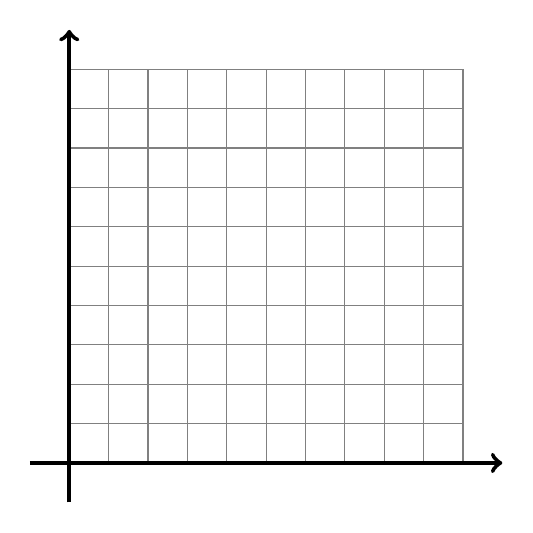
\begin{tikzpicture}
    \draw[gray] (0,0) grid[step=0.5cm] (5,5);
    \draw[ultra thick,black,->] (-0.5,0) -- (5.5,0);
    \draw[ultra thick,black,->] (0,-0.5) -- (0,5.5);

  \end{tikzpicture}
  \caption{Auswirkungen verschiedener Lernraten}
\end{figure}

\subsubsection{Stochastisches Gradientenverfahren fuer Machine Learning}
Wie vorhin erklaert, wird fuer das Trainieren eines Modells das Gradientenverfahren benutzt.
Konkret wird die Kostenfunktion $C(\vec{y},\vec{\hat{y}}|\hyperp_0,\ldots,\hyperp_n)$
($\hyperp$ sind die Modellparameter, $\vec{y}$ die Vorhersagen und $\vec{\hat{y}}$
die Labels) minimieren, indem die Parameter angepasst werden. Dadurch macht das Modell immer bessere Vorhersagen.
Fuer nur eine Iteration des Gradientenverfahren, muesste man den Gradienten fuer den
\textit{gesamten} Trainingsdatensatz berechnen.
Dies waere zwar ein exakter Prozess, aber ein extrem langsamer zugleich.
Bei grossen Datensaetzen wuerde es eine Ewigkeit dauern, bis das Modell nur annahernd guete Vorhersagen machen wuerde.
\para{}
Aus diesem Grund verwendet man eine leicht abgeänderte Variante dieses Verfahren, naemlich das \keyword{Stochastische Gradientenverfahren} (engl.: Stochastic Gradient Descent).
Hierfuer wird der ``echte'' Gradient des gesamten Datensatzes mit dem Gradienten einiger Trainingsbeispiel approximiert.
Dazu wird der Trainingsdatensatz in sogennante \keyword{Mini-Batches} eingeteilt und der Gradient jeweils pro Mini-Batch berechnet.
Als Konsequenz finden deutlich mehr Iterationen statt in \textit{einer}
Durchkaemmung der Trainingsdaten, welche man als \keyword{Epoche} bezeichnet. Oft wird mehrere Epochen lang trainiert.
Der Gradient eines genug grossen Mini-Batches ist zwar nicht ganz exakt, aber approximiert den Gradieten des gesamten Datensatzen genuegend gut.
Sowohl die Mini-Batch Groesse, wie auch die Anzahl Epochen sind weitere Hyperparameter.
\para{}
Die partiellen Ableitungen der gesamten Trainingsdaten wird mit dem arithmetischen Mittel der partiellen Ableitungen eines Mini-Batches der Groesse $q$ approximiert. Siehe Gleichung (\ref{eq:minibatch_deriv}).
\begin{equation}\label{eq:minibatch_deriv}
  \partderiv{\bar{C}}{\hyperp_k} \approx \frac{1}{q}\sum_{i=1}^{q} \partderiv{C_i}{\hyperp_k}
\end{equation}

Eine Iteration des Stochastischen Graidentenverfahren wird analog zu Gleichung (\ref{eq:gradientdescent}) folgendermassen durchgefuehrt:
\begin{equation}\label{eq:sgd}
  \hyperp_{k,t+1} = \hyperp_{k,t} - \frac{\eta}{q} \sum_{i=1}^{q} \partderiv{C_i}{\hyperp_{k,t}}
\end{equation}


\subsubsection{Adam Optimizer}
ZUSAMMENFASSUNG TRAININGSALGORITHMUS

\pagebreak
\subsection{Künstliche Neuronale Netze und Deep Learning}
Das wohl beste Modell fuer die meisten Problemstellungen in Bereich Machinelles Lernen (Bilderkennung, Spracherkennung, etc.) ist das \keyword{Kuenstliche Neuronale Netz}, kurz KNN (eng.: Neural Network).
Die Methoden welche benutzt werden um Neuronale Netze zu traniert fasst man unter dem Begriff \keyword{Deep Learning} zusammen.

Kuenstliche Neuronale Netze sind zum Teil biologisch inspiriert von Nervensystemen von Lebewesen. Sie sind aber lediglich eine Abstraktion der Informationverarbeitung und versuchen nicht eine moeglichst genaue biologische Abbildung darzustellen.
Es gibt nicht nur eine Art von Neuralem Netz, sondern es exisitieren die
verschiedensten Architekturen, welche je nach Problemstellung ausgewaehlt werden
muessen. Diese Arbeit wird sich spaeter vorallem mit sogennanten Autoencodern auseinandersetzen.


\subsubsection{Perzeptron}
Um den Aufbau und die Funktion eines Kuenstlichen Neuronalen Netz besser zu
verstehen, wird im folgenden ein Vorgaenger des KNN erklaert: das \keyword{Perzeptron}.
\para{}
Das einlagige Perzeptron wurde erstmals 1958 von Frank Rosenblatt vorgestellt. Dieses
besteht aus einem einzigen Kuenstlichen Neuron. Dieses Kuenstliche Neuron
hat mehrere binaere Inputs und einen einzigen binaeren Output. Binaer
bedeutet, dass der Wert nur entweder 0 (\textit{aus}) oder 1 (\textit{ein}) sein
kann. Des weiteren besitzt es mehrere sogenannte \keyword{Gewichte} $w_1, \ldots,
w_n \in \set{R}$, fuer jeden Input ein Gewicht.
Diese sind reelle Zahlen, welche das Verhalten des Perzeptron bestimmen.
Die \keyword{gewichtete Summe}, also die Summe aller Produkte der Inputs mit
ihrem Gewicht, wird mit $\tilde{z}$ bezeichnet.
Sie ist das gleiche wie das Skalarprodukt des Gewichtevektor mit dem Inputvektor:
$\displaystyle \tilde{z} = \sum_{i=1}^{n} w_i x_i = \vec{w} \cdot \vec{x}$\\
Zusaetzlich besitzt das Perzeptron einen \keyword{Schwellenwert} $\tilde{b}$.
Zusammen mit den Gewichten, bildet er die Modellparameter.
Das Perzeptron verhaelt sich so, dass falls die gewichtete Summe groesser als der
Schwellwert ist, das Neuron feuert, d.h.\ der Output betraegt 1. Andernfalls ist er 0.
Siehe erster Teil der Gleichung (\ref{eq:perzeptron_1}).
Es ist gaengig die Ungleichung der Bedingung in die Nullstellenform zu bringen
und $\tilde{b}$ durch die \keyword{Neigung} (engl.: Bias)
$b = -\tilde{b}$ zu ersetzten. Somit lautet die Ungleichung: $\tilde{z} + b
> 0$. Der Term $\tilde{z} + b$ wird mit $z$ bezeichnet. Siehe Rest der Gleichung (\ref{eq:perzeptron_1}).
Die Neigung gibt an wie stark das Neuron dazu neigt zu feuern. Ein hohes $b$
laesst ein Neuron auch trotz einigen Nullen in den Inputs feuern, waehrend es
fuer ein tiefes $b$ nicht feuern lassen wuerde.

\begin{equation}\label{eq:perzeptron_1}
  p(\vec{x}) =
  \begin{cases}
    1 & \quad \text{falls } \tilde{z} > \tilde{b}\\
    0 & \quad \text{ansonsten}
  \end{cases}
  \quad =
  \begin{cases}
    1 & \quad \text{falls } \tilde{z} + b > 0\\
    0 & \quad \text{ansonsten}
  \end{cases}
  \quad =
  \begin{cases}
    1 & \quad\text{falls } \vec{w} \cdot \vec{x} + b > 0\\
    0 & \quad\text{ansonsten}
  \end{cases}
\end{equation}

\begin{figure}[h!]
  \centering
  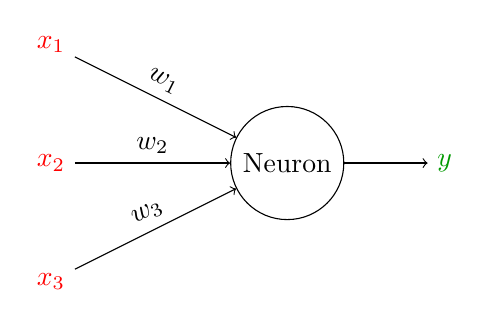
\begin{tikzpicture}
    \path (3,0) node [circle,draw](neuron){Neuron};
    \path[red] (0,1.5) node(x1){$x_1$} (0,0) node(x2){$x_2$} (0,-1.5) node(x3){$x_3$};
    \path[black!40!green] (5,0) node(y1){$y$};
    \draw[->] (x1) -- node[above,sloped]{$w_1$} (neuron);
    \draw[->] (x2) -- node[above,sloped]{$w_2$} (neuron);
    \draw[->] (x3) -- node[above,sloped]{$w_3$} (neuron);
    \draw[->] (neuron) -- (y1);
  \end{tikzpicture}
  \caption{Perzeptron mit drei Inputs}
  \label{fi:perzeptron}
\end{figure}

Fuer das Trainieren des Perzeptron existieren spezielle Verfahren, welche hier
aber nicht relevant sind. Das Gradientenverfahren kann naemlich nicht verwendet
werden. Der Grund dafuer sollte spaeter in Sektion (\ref{sec:kuenstlicheNeuronen}) einleuchtend werden.
\para{}
Nun stellt sich die Frage, was ein Perzeptron erlernen kann und wofuer es genutzt werden kann.
Das Perzeptron ist lediglich ein \keyword{Linearer Klassifikator} der Form
$y=w_1x_1+\cdots+w
_nx_n$.
Es kann die Features in zwei Klassen 0 oder 1 einordnen.
Ueberschreitet $y$ den Schwellenwert, werden die Features der Klasse 1 zugeordnet, sonst
der Klasse 0.
Jedoch muessen diese Klassen linear separierbar sein.
Das bedeutet, dass die Inputvektoren $\vec{x}$ durch eine Hyperebene trennbar
sein muessen.
Bei zwei Features (zwei Inputs) handelt es sich bei der Hyperebene um eine
Gerade welche die Vektoren auftrennt. Siehe Abbildung (\ref{fig:linearer_Klassifikator}).
Fuer drei Featuers ist es eine Ebene.
ZU ABSTRAKT -> BEISPIEL

Eine Funktionen, welche nicht linear separierbar ist (z.B\ XOR-Verknuepfungen),
kann von einem Perzeptron nicht erlernt werden.

\begin{figure}[h!]

  \caption{erfolgreiche lineare Separierung (links) und das Versagen bei XOR (rechts)}
  \label{fig:linearer_Klassifikator}
\end{figure}

\cite{wiki:perzeptron}

\subsubsection{Biologische Analogie}
SCHREIBEN
% Gewicht entscheidet ob inhibitorisch oder exaktorisch.
% Schwellenwert: Das Addieren eines Schwellenwerts  zur Netzeingabe verschiebt die gewichteten Eingaben. Die Bezeichnung bestimmt sich aus der Verwendung einer Schwellenwertfunktion als Aktivierungsfunktion, bei der das Neuron aktiviert wird, wenn der Schwellenwert überschritten ist. Die biologische Motivierung dabei ist das Schwellenpotential bei Nervenzellen. Mathematisch gesehen wird die Trennebene, die den Merkmalsraum auftrennt, durch einen Schwellenwert mit einer Translation verschoben.

% Hebbsche Lernregel

\subsubsection{Erweiterung der Kuenstlichen Neuronen}\label{sec:kuenstlicheNeuronen}
Ein Perzeptron ist, wie vorhin erklaert, nur in der Lage, lineare Klassifikationen
durchzufuehren. Um nun auch kompliziertere Probleme zu loesen, muss das Prinzip
ausgebaut werden. Ausserdem brauchen wir ein Kuenstliches Neuron, welches sich
besonders gut als Baustein fuer KNNs eignet.

\paragraph{Kuenstliche Neuronen im Allgemeinen}
Kuenstliche Neuronen sind immer so aufgebaut, dass sie einen oder mehrere Inputs
haben und einen einzigen Output. Zu jedem Input $x_i$ ist ein Gewicht
$w_{ji}$ assoziert. Zuerst wird die gewichtete Summe der Inputs $\tilde{z}$ gebildet.
Die Neigung $b$ wird ebenfalls draufaddiert, um $z$ zu erhalten. Nun muss
die sogennante Aktivierung $a$ gebildet werden. Sie entspricht dem Output des Neurons.
Die Aktivierung $a$ ist das Resultat der Aktivierungsfunktion $\varphi$ angewendet
auf $z$. $a = \varphi(z)$. Die verschiedenen Kuenstlichen Neuronen unterscheiden
sich fast nur in ihrer Aktivierungsfunktion.

\paragraph{Perzeptronen als Kuenstliche Neuronen}
Zuerst noch einmal ein Blick auf das Perzeptron in Betracht der Aktivierungsfunktion.
Ein wesentlicher Unterschied des Perzeptron gegenueber sonstigen Kuenstlichen
Neuronen, besteht darin, dass seine Inputs und Outputs nur binaere Werte
annehmen koennen. Um dieses Verhalten des Perzeptron zu erhalten,
muss eine Stufenfunktion als Aktivierungfunktion verwendet werden: die Heaviside-Funktion $\Theta$.
Sie hat einen einzigen Stufensprung bei $x=0$ vom Wert 0 auf 1. Siehe Abb. (\ref{fig:heaviside}).

\begin{figure}[h!]
  \begin{minipage}[h!]{0.5\textwidth}
    \begin{equation*}
      \varphi^{\text{hlim}}(z) = \Theta(z) =
      \begin{cases}
        1 & \quad \text{falls } z \geq 0\\
        0 & \quad \text{falls } z < 0
      \end{cases}
    \end{equation*}

  \end{minipage}
  \begin{minipage}[h!]{0.5\textwidth}
    \centering
    \begin{tikzpicture}[scale=2.5]

      \draw[->] (-1.5,0) -- (1.5,0) node[right] {$x$}; % x-axes
      \draw[->] (0,-0.2) -- (0,1.2) node [above] {$y$}; % y-axes
      \draw[style=help lines,step=0.5] (-1.4,0) grid (1.4, 1.1);

      \foreach \x in {-1,-0.5,0.5,1}
      \draw[shift={(\x,0)}] (0pt,2pt) -- (0pt,-2pt) node[below,fill=bgcolor] {$\x$};

      \foreach \y in {0.5,1}
      \draw[shift={(0,\y)}] (2pt,0pt) -- (-2pt,0pt) node[left,fill=bgcolor] {$\y$};

      \draw[shift={(0,0)}] (0pt,0pt) node[below left,fill=bgcolor] {$O$};

      \draw[red,ultra thick] (-1.5,0) -- (0,0); % 0-red
      \draw[red,ultra thick] (0,1) -- (1.5,1); % 1-red
      \draw[red,ultra thick,dashed] (0,0) -- (0,1); % y-red
      \draw[draw=red,fill=white] (0,0) circle (0.05);
      \draw[draw=red,fill=red] (0,1) circle (0.05);

    \end{tikzpicture}
  \end{minipage}

  \caption{Definition und Graph der Heaviside-Funktion $\Theta$}
  \label{fig:heaviside}
\end{figure}

\paragraph{Stueckweise lineare Neuronen}
Der naechste Schritt nach dem binaeren Perzeptron sind sogenannte stueckweise
lineare Neuronen.
Sie verwenden eine stueckweise lineare Aktivierungsfunktion. Diese bildet ein
beschraenktes Intervall linear ab. Die Werte ausserhalb werden auf die
konstanten Werte 0 oder 1 abbgebildet. Siehe Abb. (\ref{fig:stueckweiselinear}).
\para{}
Die Inputs koennen jetzt beliebige reelle Zahlen sein (vorzugsweise in der Naehe
von 0 und 1).
Ein KNN aus ausschliesslich linearen Neuronen ist ziemlich nutzlos, da jedliche Verkettung von
linearen Funktion auch durch eine einzige lineare Funktion dargestellt werden
koennte. Somit hat ein KNN gegenueber einem einzelnen Neuron keinen Mehrwert.
Ausserdem koennen mit diesen Neuron auch nur lineare Probleme geloest werden.

\begin{figure}[h!]
  \begin{minipage}[h!]{0.5\textwidth}
    \begin{equation*}
      \varphi^{\text{pwl}}(z) =
      \begin{cases}
        1 & \quad \text{falls } z > \frac{1}{2}\\
        z + \frac{1}{2} & \quad \text{falls } -\frac{1}{2} < z < \frac{1}{2}\\
        0 & \quad \text{falls } z < \frac{1}{2}
      \end{cases}
    \end{equation*}

  \end{minipage}
  \begin{minipage}[h!]{0.5\textwidth}
    \centering
    \begin{tikzpicture}[scale=2.5]

      \draw[->] (-1.5,0) -- (1.5,0) node[right] {$x$}; % x-axes
      \draw[->] (0,-0.2) -- (0,1.2) node [above] {$y$}; % y-axes
      \draw[style=help lines,step=0.5] (-1.4,0) grid (1.4, 1.1);

      \foreach \x in {-1,-0.5,0.5,1}
      \draw[shift={(\x,0)}] (0pt,2pt) -- (0pt,-2pt) node[below,fill=bgcolor] {$\x$};

      \foreach \y in {0.5,1}
      \draw[shift={(0,\y)}] (2pt,0pt) -- (-2pt,0pt) node[left,fill=bgcolor] {$\y$};

      \draw[shift={(0,0)}] (0pt,0pt) node[below left,fill=bgcolor] {$O$};

      \draw[red,ultra thick] (-1.5,0) -- (-0.5,0); % 0-red
      \draw[red,ultra thick] (0.5,1) -- (1.5,1); % 1-red
      \draw[red,ultra thick] (-0.5,0) -- (0.5,1); % d-red

      \draw[draw=red,fill=red] (-0.5,0) circle (0.03);
      \draw[draw=red,fill=red] (0.5,1) circle (0.03);


    \end{tikzpicture}
  \end{minipage}

  \caption{Formel und Graph einer stueckweisen linearen Funktion}
  \label{fig:stueckweiselinear}
\end{figure}


\paragraph{Sigmoide Neuronen}
Die logische naechste Erweiterung sind nicht-lineare Neuronen.
Ein sehr beliebter Kandidat dafuer sind Sigmoide Neuronen.
Den Namen haben sie von ihrer Aktivierungsfunktion: der Sigmoidfunktion $\sigma$.
Eine sehr wichtige Eigenschaft von ihr ist, dass sie - im Gegensatz zu den vorhin
genannten Aktivierungsfunktion - ueberall differenzierbar und strikt monoton
steigend ist. Erst fuer diese Aktivierungsfunktion, kann das Gradientenverfahren
angewendet werden und somit das KNN trainiert werden. Die anderen
Funktionen haben Stellen bei welchen die Ableitungsfunktion null
betraegt, somit kann das lokale Minimum nicht gefunden werden.
Nicht nur die Sigmoidfunktion erfuellt diese Bedingungen, sondern auch andere. Die Sigmoidfunktion wird
bevorzugt, da ihre Ableitung sehr simpel ist, siehe Abb. (\ref{fig:sigmoid}).
Die Nicht-linearitaet dieser Neuronen ermoeglicht ein Erlernen von deutlich komplexeren Sachverhalten.
Und wie spaeter in Sektion (\ref{sec:UAT}) erlautert, ist es moeglich mit der Kompostion von nicht-linearen
Funktionen jede belibige Funktion zu approximieren!
\para{}
Die Simgmoid-Funktion besitzt eine einzige Wendestelle bei $x=0$ und hat zwei Asymptoten, eine fuer $x \to -\infty$ mit $y=0$
und eine zweite fuer $x \to\infty$ mit $y=1$. Siehe Abb. (\ref{fig:sigmoid}).

\begin{figure}[h!]
  \begin{minipage}[h!]{0.5\textwidth}
    \begin{align*}
      \varphi^{\text{sig}}(z) &= \sigma(z) = \frac{1}{1 + e^{-z}}\\
      \sigma'(z)&=\sigma(z)(1-\sigma(z))
    \end{align*}
  \end{minipage}
  \begin{minipage}[h!]{0.5\textwidth}
    \centering
    \begin{tikzpicture}[scale=2.5]

      \draw[->] (-1.5,0) -- (1.5,0) node[right] {$x$}; % x-axes
      \draw[->] (0,-0.2) -- (0,1.2) node [above] {$y$}; % y-axes
      \draw[style=help lines,ystep=0.5,xstep=0.25] (-1.4,0) grid (1.4, 1.1);

      \foreach \x/\xtext in {-1/-4,-0.5/-2,0.5/2,1/4}
      \draw[shift={(\x,0)}] (0pt,2pt) -- (0pt,-2pt) node[below,fill=bgcolor] {$\xtext$};

      \foreach \y in {0.5,1}
      \draw[shift={(0,\y)}] (2pt,0pt) -- (-2pt,0pt) node[left,fill=bgcolor] {$\y$};

      \draw[shift={(0,0)}] (0pt,0pt) node[below left,fill=bgcolor] {$O$};


      \draw[red,ultra thick,x=0.25cm] plot[domain=-6.0:6.0] (\x,{1/(1+exp(-\x)) });

    \end{tikzpicture}
  \end{minipage}

  \caption{Definition, Ableitung und Graph der Sigmoid-Funktion $\sigma$}
  \label{fig:sigmoid}
\end{figure}




\subsubsection{Topologie der Kuenstlichen Neuronalen Netzen}
Nun sollten diese Sigmoiden-Neuronen als Bausteine verwendet werden, um ein Kuenstliches
Neuronales Netz zu bilden. Dazu werden sie miteinander verbundet und bilden so ein Netz,
aehnlich wie ein Nervensystem.
Diese Neuronen sind in verschieden Schichten (engl.: Layers)
arangiert. Die erste ist die \keyword{Inputschicht}. Sie behinhalten die
Inputneuronen. Dies sind eigentlich keine richtigen
Neuronen sondern eher Platzhalter fuer ihren jeweiligen Inputwert $x_i$. Als letztes kommt die
\keyword{Outputschicht} mit den Outputneuronen, welche jeweils einen Outputwert $y_i$
besitzen. Dazwischen liegen die \keyword{Zwischenschichten} (engl.: Hiddenlayer). Von ihnen kann es
beliebig viele geben und in ihnen beliebig viele Neuronen.
Der Aufbau eines KNN bezeichnet man als \keyword{Topologie} des Netzes. Die
Topologie umfasst viele Hyperparameter. Darunter sind zum Beispiel die Anzahl Zwischenschichten, wie auch
die Anzahl Neuronen pro Schicht.
\para{}
Jedes Neuron aus einer Schicht ist mit jedem Neuron aus der naechsten Schicht ueber
Verbindungen gekoppelt. Alle Verbindungen besitzten ein Gewicht analog zu den Inputs des
Perzeptron. Die Aktivierung, also der Output, eines Neurons wandert entlang den jeweiligen
Verbindung zu allen Neuronen der naechsten Schicht und dient als deren Input.
Die soeben beschriebe Art von KNN nennt man \keyword{Feedforward-Netz}, da alle Werte
ausschliesslich nach vorne propagiert werden.

In Abbildung (\ref{fi:nn_layers}) ist ein Beispiel eines Neuronalen Netzes
abgebildet. In diesem Fall besitz es sowohl 4 Inputs, wie auch 4 Outputs. Es hat
ausserdem 3 Zwischenschichten. Die zwei aueserren Zwischenschichten haben 3 Neuronen und die dazwischen
hat sogar 4 Neuronen.
\\ABBILDUNG MIT BESCHRIFTUNG DER GEWICHTE

\begin{figure}[h!]
  \centering
  \begin{tikzpicture}[>=latex]

    \tikzstyle{netstyle} = [matrix of nodes,nodes={draw,circle,inner sep=0, minimum size=1cm},column sep=0.5cm,row sep=-9pt]
    \tikzstyle{cl} = [draw=none,fill=none]
    \tikzstyle{heading} = [clear,text width=15mm,text centered]
    \tikzstyle{inp} = [fill=red!70!bgcolor]
    \tikzstyle{hid} = [fill=blue!70!bgcolor]
    \tikzstyle{ou} = [fill=green!70!bgcolor]

    \matrix[netstyle] (mat)
    {
      |[inp]| $x_1$     & |[cl]| & |[cl]| & |[hid]|$h_1^2$ & |[cl]| & |[cl]| & |[ou]|$y_1$ \\
      |[cl]| & |[cl]| & |[hid]|$h_1^1$   & |[cl]| & |[hid]|$h_1^3$ & |[cl]| & |[cl]| \\
      |[inp]| $x_2$     & |[cl]| & |[cl]| & |[hid]|$h_2^2$ & |[cl]| & |[cl]| & |[ou]|$y_2$ \\
      |[cl]| & |[cl]| & |[hid]|$h_2^1$   & |[cl]| & |[hid]|$h_2^3$ & |[cl]| & |[cl]| \\
      |[inp]| $x_3$     & |[cl]| & |[cl]| & |[hid]|$h_3^2$ & |[cl]| & |[cl]| & |[ou]|$y_3$ \\
      |[cl]| & |[cl]| & |[hid]|$h_3^1$   & |[cl]| & |[hid]|$h_3^3$ & |[cl]| & |[cl]| \\
      |[inp]| $x_4$     & |[cl]| & |[cl]| & |[hid]|$h_4^2$ & |[cl]| & |[cl]| & |[ou]|$y_4$ \\
    };

    % titels
    \node [yshift=1cm] at (mat-1-1) {Inputschicht};
    \node [yshift=1cm] at (mat-1-4) {Zwischenschichten};
    \node [yshift=1cm] at (mat-1-7) {Outputschicht};

    % dots
    % \node [yshift=-1cm,scale=2] at (mat-7-1) {$\vdots$}; % for inputs
    % \node [yshift=-1cm,scale=2] at (mat-6-3) {$\vdots$};
    % \node [yshift=-1cm,scale=2] at (mat-7-4) {$\vdots$};
    % \node [yshift=-1cm,scale=2] at (mat-6-5) {$\vdots$};
    % \node [yshift=-1cm,scale=2] at (mat-7-7) {$\vdots$}; % for outputs

    % input -> hidden1
    \foreach \ai in {1,3,...,7} {
      \foreach \aii in {2,4,6}
      \draw[->] (mat-\ai-1) -- (mat-\aii-3);
    }

    % hidden1 -> hidden2
    \foreach \ai in {2,4,...,6} {
      \foreach \aii in {1,3,...,7}
      \draw[->] (mat-\ai-3) -- (mat-\aii-4);
    }

    % hidden2 -> hidden3
    \foreach \ai in {1,3,...,7} {
      \foreach \aii in {2,4,6}
      \draw[->] (mat-\ai-4) -- (mat-\aii-5);
    }

    % hidden3 -> output
    \foreach \ai in {2,4,...,6} {
      \foreach \aii in {1,3,...,7}
      \draw[->] (mat-\ai-5) -- (mat-\aii-7);
    }

  \end{tikzpicture}
  \label{fi:nn_layers}
  \caption{Schichten eines KNNs}
\end{figure}

\subsubsection{Vorwaertspropagierung}
Jetzt, da der Aufbau eines KNNs erklaert wurde, sollte nun die mathematische Funktionsweise
des Modells erklaert werden. Hierfuer muessen einige Konventionen zur
Bezeichnung der Teile eines KNNs getroffen werden:

\begin{itemize}

\item{$n_j^l$ ist das $j$-te Neuron in der $l$-ten Schicht.}
\item{$z_j^l$ ist die gewichtete Summe der Inputs des $j$-ten Neuron in der $l$-ten Schicht.}
\item{$a_j^l$ ist die Aktivierung des $j$-ten Neurons in der $l$-ten Schicht.}
\item{$b_j^l$ ist die Neigung des $j$-ten Neuron in der $l$-ten Schicht.}
\item{$w_{j,k}^l$ ist das Gewicht der Verbindung vom $k$-ten Neuron
    in der ($l-1$)-ten Schicht zum $j$-ten Neuron in der $l$-ten Schicht (man
    beachte die Reihenfolge)
    \footnote{
      Diese Konvention scheint auf den ersten Blick unintuitiv, macht jedoch
      Sinn fuer die spaeteren mathematischen Operationen mit Matrizen in Sektion
      (\ref{sec:backpropagation}).
    }.}

\item{$L$ soll die gesamte Anzahl der Schichten sein.}

\item{$N_l$ ist die Anzahl Neuronen in der $l$-ten Schicht.}

\item{$\varphi$ ist die gewaehlte Aktivierungsfunktion (grundsaetzlich ist diese
    immer die Sigmoidfunktion $\sigma$).}

\end{itemize}

ABBILDUNG MIT GEWICHTEBESCHRIFTUNGEN (KORREKT!)
\begin{figure}[h!]
  \centering
  \begin{tikzpicture}[>=latex]

    \tikzstyle{netstyle} = [matrix of nodes,nodes={draw,circle,inner sep=0, minimum size=1.25cm},column sep=0.5cm,row sep=-9pt]
    \tikzstyle{cl} = [draw=none,fill=none]
    \tikzstyle{sy} = [cl,font=\LARGE]
    \tikzstyle{heading} = [clear,text width=15mm,text centered]
    \tikzstyle{inp} = [fill=red!70!bgcolor]
    \tikzstyle{hid} = [fill=blue!70!bgcolor]
    \tikzstyle{ou} = [fill=green!70!bgcolor]

    \matrix[netstyle] (mat)
    {
      |[inp]|$a_1^0$     & |[cl]| & |[cl]| & |[cl]| & |[cl]| & |[cl]| & |[ou]|$a_1^L$ \\
      |[cl]| & |[cl]| & |[hid]|$a_1^1$   & |[sy]| $\cdots$ & |[hid]|$a_1^{L-1}$ & |[cl]| & |[cl]| \\
      |[inp]|$a_2^0$     & |[cl]| & |[cl]| & |[cl]| & |[cl]| & |[cl]| & |[ou]|$a_2^L$ \\
      |[cl]| & |[cl]| & |[hid]|$a_2^1$   & |[sy]| $\cdots$ & |[hid]|$a_2^{L-1}$ & |[cl]| & |[cl]| \\
      |[inp]|$a_3^0$     & |[cl]| & |[sy]| $\vdots$ & |[cl]| & |[sy]| $\vdots$ & |[cl]| & |[ou]|$a_3^L$ \\
      |[sy]| $\vdots$ & |[cl]| & |[hid]|$a_{N_1}^1$ & |[sy]|$\cdots$ & |[hid]|$a_{N_{L-1}}^{L-1}$ & |[cl]| & |[sy]| $\vdots$ \\
      |[inp]|$a_{N_0}^0$ & |[cl]| & |[cl]| & |[cl]| & |[cl]| & |[cl]| & |[ou]|$a_{N_L}^L$ \\
    };

    % titels
    \node [yshift=1.5cm] at (mat-1-1) {Inputschicht};
    \node [yshift=1.5cm] at (mat-2-4) {Zwischenschichten};
    \node [yshift=1.5cm] at (mat-1-7) {Outputschicht};

    % input -> hidden1
    \foreach \ai in {1,3,...,7} {
      \foreach \aii in {2,4}
      \draw[->] (mat-\ai-1) -- node[above,sloped]{$w_{\aii,\ai}^1$} (mat-\aii-3);
    }

    % hidden1 ->...
    \foreach \ai in {2,4,...,6} {
      \foreach \aii in {2,4,...,6} {
        \node (A) at (mat-\ai-3) {};
        \node (B) at (mat-\aii-5) {};
        \draw[left color=black,right color=white] (mat-\ai-3) -- ($(A)!0.3!(B)$);
      }
    }

    % ...-> hidden2
    \foreach \ai in {2,4,...,6} {
      \foreach \aii in {2,4,...,6} {
        \node (A) at (mat-\ai-3) {};
        \node (B) at (mat-\aii-5) {};
        \draw[left color=black,right color=white] ($(A)!0.7!(B)$) -- (mat-\aii-5);
      }
    }

    % hidden3 -> output
    \foreach \ai in {2,4,...,6} {
      \foreach \aii in {1,3,...,7}
      \draw[->] (mat-\ai-5) -- node[above,sloped]{$w_{\aii,\ai}^L$} (mat-\aii-7);
    }

  \end{tikzpicture}
  \label{fi:nn_layers}
  \caption{zum Verstaentniss der Nomenklatur}
\end{figure}

\par\bigskip
Die Vorwaertspropagierung beginnt bei den Inputneuronen, welche jeweils
einen Inputwert in sich tragen. Diese werden, um fuer eine kohaerente Nomenklatur zu sorgen,
gleich wie die Aktivierungen der anderen Neuronen mit $a_j^0$ bezeichnet, wobei
$j$ der Index des Neurons ist.\par
Nun muessen die restlichen Aktivierungen der Neuronen berechnet werden. Dies geschieht rekursiv, anhand der
Aktivierungen der voherigen Schicht. Und zwar folgendermassen (ersichtlich in
Gleichung (\ref{eq:gewichtete_summe_normal})):\par
Zuerst laueft eine Summe ueber alle Neuronen $n_k^{l-1}$ der voherigen Schicht
($l-1$). Dabei wird die gewichtete Summe der Aktivierungen $a_k^{l-1}$ mit den
assozierten Gewichten $w_{j,k}^l$ gebildet. Hierbei ist das Gewicht jenes, welches das
$k$-te Neuron der ($l-1$)-ten Schicht mit dem $j$-ten Neuron der $l$-ten Schicht verbindet.
Zusaetzlich gehoert zu der gewichteten Summe auch die jeweilige Neigung $b_j^l$, welche
dazuaddiert wird. Diese gewichtete Summe wird mit $z_j^l$ bezeichnet.

\begin{equation}\label{eq:gewichtete_summe_normal}
  z_j^l = \sum_{k=1}^{N_l} w_{j,k}^l a_k^{l-1} + b_j^l
\end{equation}

Auf diese Summe wird dann die Aktivierungsfunktion $\varphi$ angewandt.
Das ist dann die Aktivierung $a_j^l$ des Neurons.

\begin{equation}\label{eq:aktivierung_normal}
  a_j^l = \varphi\left(\sum_{k=1}^{N_l} w_{j,k}^l a_k^{l-1} + b_j^l \right) = \varphi \left( z_j^l \right)
\end{equation}
\par\bigskip
Da KNNs weit verbreitet sind in der Bilderkennung und Spracherkennung, ist es
nicht unueblich, dass diese sehr viele Neuronen und Verbindungen (ueber 100'000) besitzen.
Um hierbei nicht den Ueberblick zu verlieren und um nicht in den Indizes zu
ertrinken, greift man auf \keyword{Lineare Algebra} zurueck. Man verwendet
Matrizen und Vektoren um die vielen Variabeln zusammen zu fassen.
Ausserdem besteht ein weiterer Vorteil darin, dass Computer mithilfe von Vektor-
und Matrixoperationen die Berechnungen parallisieren koennen und in kuerzerer
Zeit und mit weniger Ressourcen viele Brechnungen gleichzeitig ausfuehren koennen.
Dies beschleunigt das Training der Modelle um
ein Vielfaches. Dies wird spaeter in Sektion
(\ref{sec:tensorflow}) noch weiter thematisiert.
\para{}
Die Inputs $\vec{x}$, Outputs $\vec{y}$ und Labels $\vec{\hat{y}}$ haben wir schon von Anfang an als Vektoren geschrieben.
Nun sollen noch die Parameter und die restlichen Komponenten eines KNNs als Vektoren und Matrizen geschrieben werden.
Sowohl alle gewichteten Summen $z_j^l$, wie auch alle Aktivierungen $a_j^l$
einer Schicht $l$, werden in Vektoren $\vec{z}^l$ und $\vec{a}^l$ zusammengefasst.
Alle Neigung $b_j^l$ einer Schicht $l$ bildet ebenfalls eines Vektor $\vec{b}^l$.
Zu guter letzt, wird noch eine \keyword{Gewichtsmatrix} $\mat{W}^l$ fuer jede
Schicht $l$ definiert.
Die Eintraege dieser Matrix sind einfach die Gewichte welche \textit{zu} den Neuronen der
$l$-ten Schicht verlaufen. Das heisst der Eintrag in der $j$-ten Zeile und in
der $k$-ten Spalte ist $w_{j,k}^l$ (Siehe Gl. (\ref{eq:gewichtsmatrix})).

\begin{equation}\label{eq:gewichtsmatrix}
  \mat{W}^l =
  \begin{pmatrix}
    w_{1,1}^l & w_{1,2}^l & \cdots & w_{1,n}^l \\[0.3em]
    w_{2,1}^l & w_{2,2}^l & \cdots & w_{2,n}^l \\[0.3em]
    \vdots & \vdots & \ddots & \vdots \\[0.3em]
    w_{m,1}^l & w_{m,2}^l & \cdots & w_{m,n}^l
  \end{pmatrix}
\end{equation}

Mit diesen Definitionen kann nun Gleichung (\ref{eq:aktivierung_normal}) in
Matrixform geschrieben werden. Hierfuer muss noch ein weiteres mathematisches
Konzept eingefuehrt werden: die Vektorisierung einer Funktion.
\para{}


\begin{defbox}{Vektorisierung einer Funktion}
  Die Vektorisierung einer Funktion $f$, geschrieben als $f[\vec{v}]$ ist eine
  neue Funktion, welche als Rueckgabewert einen Vektor hat, auf dessen
  Komponenten jeweils immer die Funktion $f$ angewendet wird.
  \begin{equation*}
    f[\vec{v}]=
    \begin{pmatrix}
      f(v_1)\\
      \vdots \\
      f(v_n)\\
    \end{pmatrix}
  \end{equation*}
\end{defbox}

\para{}

Nun kann die Matrixschreibweise eingefuehrt werden (siehe Gleichung (\ref{eq:aktivierung_matrix})).\par
Zuerst wird eine Matrixmultiplikation der Gewichtsmatrix $\mat{W}^l$ mit dem
Aktivierungsvektor $\vec{a}^{l-1}$ der vorherigen Schicht durchgefuehrt. Darauf
wird der Neigunsvektor addiert. Und zu guter Letzt wird die vektorisierte
Aktivierungsfunktion $\varphi$ angewandt.
\begin{equation}\label{eq:aktivierung_matrix}
  \vec{z}^{\,l} = \mathbf{W}^{\,l} \vec{a}^{\,l-1} + \vec{b}^{\,l}
\end{equation}
\par
\begin{equation}\label{eq:aktivierung_matrix}
  \vec{a}^{\,l} = \varphi \left[\mat{W}^{\,l} \vec{a}^{\,l-1} + \vec{b}^{\,l} \right] = \varphi \left[ \vec{z}^l \right]
\end{equation}


\subsubsection{Gewichte und Neigungen initalisieren*}

\subsubsection{Rueckwaertspropagierung}\label{sec:backpropagation}
Die wahre Herausforderung besteht beim Gradientenverfahren darin,
die partiellen Ableitungen der Modellparameter,
also die Komponenten des Gradienten, zu bestimmen.
Anderst gesamt muessen alle
$\ipartderiv{C}{w_{j,k}^l}$ wie auch alle $\ipartderiv{C}{b_k^l}$
berechnet werden.
Das Verfahren zum bestimmen dieser Ausdruecke ist so spezfisch und aufwendig,
dass das Gradientenverfahren fuer KNNs einen eigen Namen hat: die
\keyword{Rueckwaertspropagierung} (engl.: Backpropagation).

Das Ziel dieses Algorithmus ist es die beiden Partiellen Ableitungen
$\ipartderiv{C}{w_{j,k}^l}$ und $\ipartderiv{C}{b_j^l}$
zu bestimmen. Hierfuer ist es sinnvoll eine Zwischenwert, welchen wir Fehler
$\delta_j^l$ nennen.

\para{}
\begin{defbox}{Hadamard-Produkt}
  Das Hadamard-Produkt ist ein spezielles Produkt zweier gleichgrossen Matrizen.
  Die resultierende Matrix ergibt sich aus der elementweisen Multiplikation der Ausgangsmatrizen.

  \begin{minipage}{0.5\textwidth}
    \begin{equation*}
      \mat{A} \odot \mat{B} =
      \begin{pmatrix}
        a_{1,1} b_{1,1} & \cdots & a_{1,n} b_{1,n} \\[0.3em]
        \vdots & \ddots & \vdots \\[0.3em]
        a_{m,1} b_{m,1} & \cdots & a_{m,n} b_{m,n} \\[0.3em]
      \end{pmatrix}
      \in \set{R}^{m \times n}
    \end{equation*}
  \end{minipage}
  %
  \begin{minipage}{0.5\textwidth}
    \begin{equation*}
      \vec{v} \odot \vec{w} =
      \begin{pmatrix}
        v_1 w_1 \\
        \vdots \\
        v_n w_n
      \end{pmatrix}
    \end{equation*}

  \end{minipage}
\end{defbox}
\para{}

\begin{equation}
  \delta_j^l \coloneqq \partderiv{C}{z_j^l}
\end{equation}

Viel Kettenregel.

\begin{equation}
  \partderiv{C}{w_{j,k}} = \partderiv{C}{a_k} \partderiv{a_k}{z_k} \partderiv{z_k}{w_{j,k}}
\end{equation}

Die vier magischen Gleichungen:

Der Fehler in der Outputschicht
\begin{equation}\tag{BP1}
  \delta_j^L = \partderiv{C}{a_j^L} \sigma'(z_j^L)
\end{equation}

Matrixform
\begin{equation}\tag{BP1a}
  \delta^L = \nabla_{\vec{a}}C \odot \sigma'(z^L)
\end{equation}
Das tiefgestellte $_a$ des Nablas, gibt an, dass es sich um den Gradienten mit den partiellen
Ableitungen bezueglich den Aktivierungen $a$ handelt.

Fehler anhand des Fehlers der naechsten Schicht
\begin{equation}\tag{BP2}
  \delta^l = (\trans{(w^{l+1})} \delta^{l+1}) \odot \sigma'(z^l)
\end{equation}

\begin{equation}\tag{BP3}
  \partderiv{C}{b_j^l} = \delta_j^l
\end{equation}

\begin{equation}\tag{BP4}
  \partderiv{C}{w_{j,k}^l} = a_k^{l-1} \delta_j^l
\end{equation}



\subsubsection{Universal Approximation Theorem}\label{sec:UAT}
Neural Network kann alles erlernen

\pagebreak
\subsection{Convolutional Neural Networks}
Viele Anwendungen von Machine Learning sind verbunden mit Bild- oder
Audioverarbeitung, wie z.B Bildklassifizierung, Gesichtserkennung oder
Spracherkennung.
Vorallem aber fuer hochaufloesende Bilder sind die KNNs, die wir soeben
kennengelernt haben, nicht geeignet. Sie sind zum Teil gar nicht in der
Lage eine Korrelation zwischen den Inputs und Outputs zu erlernen.
Um diesen Umstand zu erklaeren, wird nun ein kleines Beispielmodell erlauetert:
\para{}
Es soll ein KNN designed werden, welches einer Photographie danach klassifizieren
soll, ob darauf ein Hund sichtbar ist oder nicht. Wir nehmen fuer dieses
Beispiel bereits ein relativ niedrig aufgeloestes Bild mit $256 \times 256$
Pixel, dies entspricht weniger als $0.07$ Megapixel (ein iPhone XS hat eine Kamera mit
12 Megapixel). Um die verschiedenen Farben zu codieren besitzt jeder Pixel drei Komponten R, G
und B. Somit hat dieses Bild insgesamt $256 \times 256 \times 3 = 196'608$
Komponenten. Jede Komponente ist ein Feature welches das KNN zu verrechnen hat. Somit bestuende
die erste Schicht des Netzwerkes aus fast $200'000$ Neuronen. Um diese Schicht
nun mit seiner Nachbarsschicht, welche gleiche Dimensionen besitzt, zu verbinden, braucht
es $196'608 \times 196'608 = 38'654'705'664$ Verbindungen und damit gleich so
viele Gewichte! Fuer ein Netwerke ohne eine einzige Zwischenschichten gaebe es
also ueber 38 Milliarden Modellparameter zu erlernen! Das dies nicht realistisch ist,
sollte auf der Hand liegen.
\para{}
Nun sollte klar sein, dass eine andere Modellarchitektur noetig ist, um Machine
Learning auf Bilder anzuwenden. Fuer genau solche Anwendungen wurde eine modifizierte
Version eines KNNs entwickelt: das \keyword{Convolutional Neural Network} (CNN).
Diese Art von Netzwerk, macht Gebrauch von Konzepten aus der klassischen
Bildverarbeitung, wie sie mit beispielsweise Photoshop gemacht werden kann.
Wie beim Perzeptron und bei den klassischen KNNs auch, ist die Architektur
biologisch inspiriert.
Der folgende Abschnitt wird die Funktionsweise eines solchen CNNs erklaeren.
\para{}
\cite{deeplearning.ai:cnn}

\subsubsection{Bilder als 3D-Matrizen}
Bei der Betrachtung von Bildern fuer Machine Learning, ist es sinnvoll, diese
nicht als eine Anordnung von verschieden farbigen Pixeln zu interpretieren,
sondern sie als \keyword{3D-Matrizen} zu untersuchen.


\begin{defbox}{3D-Matrix}
  Eine 3D-Matrix ist ein mathematischen Objekt und eine Erweiterung von Matrizen
  auf 3-dimensionale Zahlenanordnung. Vorstellen kann man sich eine 3D-Matrix
  als ein Volumen dass Zahlen in einem Raster angeordnet hat.
  Die Zahlen sind dabei die Elemente der Matrix. Analog zum Volumen, bezeichnet
  man die Form der Matrix mit Hoehe, Breite und Tiefe.
  Eine Matrix von der Form $3 \times 3 \times 3$ koennte folgendermassen aussehen:

  TIKZPICTURE EINER 3D-Matrix

\end{defbox}

\para{}
Ein Bild kann somit einfach als 3D-Matrix, bezeichnet mit $\mat{B}_{h \times w
  \times c}$ der Form $(\text{Bildhoehe} \times
\text{Bildbreite} \times \text{Anzahl Farbkomponenten})$ betrachtet werden. Die
Elemente der Matrix nehmen dann einfach die Werte der Pixelkomponenten an.
Ein schwarzweiss Bild hat nur eine Komponente, welche die Helligkeit angibt.
Somit waere es eine normale 2D-Matrix $\mat{B}_{h \times w}$.
Siehe Abb. (\ref{fig:bildmatrix}).
\para{}
Eine solche \keyword{Bildmatrix} stellt dann den Input $\mat{X}$ eines CNNs dar und nicht mehr wie
voher ein Vektor $\vec{x}$.


\begin{figure}[h!]
  \begin{tikzpicture}

  \end{tikzpicture}
  \caption{Beispiel einer Bildmatrix}
  \label{fig:bildmatrix}
\end{figure}

\begin{figure}

  \caption{2-dimensionalen Schicht von Neuronen}
\end{figure}

\subsubsection{Filter}
\paragraph{Filter in der Bildverarbeitung}
\keyword{Filter} (engl. auch: Kernel) sind in der Bildverarbeitung sehr verbreitet. Jeder kennt sie entweder
von Photoshop, von Instagram oder sonstigen Bildbearbeitungsprogrammen.
Auch CNNs machen Gebrauch von solchen Filtern, in diesem Fall um die Features eines Bildes zu
erlernen. Aus diktaktischen Gruenden betrachten wir zuerst nur 2D-Filter, welche sich fuer graustufige
Bilder $\mat{B}_{h \times w}$ eignen.
\begin{figure}[h!]

  \caption{der Instagramfilter: Blablabla}
\end{figure}

\para{}
Filter sind einfach Regionen, deutlich kleiner als das verarbeitete Bild, welche
ueber alle Pixel wandert und diese manipuliert und so wieder ein neues Bild
$\mat{B}^*$ liefern.
Mathematisch gesehen handelt es sich bei einem Filter einfach um eine Matrix,
die sogennante \keyword{Filtermatrix} oder Faltungsmatrix (siehe Abb. (\ref{fig:filtermatrix})),
bezeichnet mit $\mat{F}_{f \times f}$. Solche Filter sind immer quadratisch,
wobei ihre Zeilen- bzw. Spaltenlaenge mit $f$ bezeichnet wird. Dabei ist $f$
immer eine ungerade Zahl, damit ein Element, das sogennante \keyword{Zentralelement}, immer im Zenturm des Filters liegt.

\begin{figure}[h!]

  \caption{eine Filtermatrix}
  \label{fig:filtermatrix}
\end{figure}
\para{}
Das Verhalten des Filters wird durch seine Matrixeintraege bestimmt.
Die Elemente koennen also so gewaehlt werden, dass wenn der Filter auf ein Bild
angewandt wird, er bestimmte Features aus dem Bild hervorhebt. Solche Features
koennten zum Beispiel Raender oder Kanten sein, welche betont werden.
\para{}
Ein gutes Beispiel ist der Sobel-Filter. Er ist ein typischer Kantendetektions-Filter mit einer
Groesse von $f = 3$. Wir betrachten nun den Sobelfilter $\mat{G}_x$, welcher
horizontale Kanten akzentuiert. Die Eintraege dieses Filters lauten wie folgt:
\begin{equation*}
  \mat{G}_x =
  \begin{bmatrix}
    -1 & 0 & +1 \\
    -2 & 0 & +2 \\
    -1 & 0 & +1 \\
  \end{bmatrix}
\end{equation*}

Angewandt auf ein Bild, erhaelt man ein neues Bild, bei welchem alle Bereiche
schwarz sind und die erkannten Kanten weiss eingefaerbt sind. Der Filter erkennt
dabei jede Stelle als Kante, welche zwei Regionen mit genug grossem Kontrast
voneinander trennt.
In Abbildung (\ref{fig:sobel_filter}) wurde der horizontale Sobelfilter auf ein
Beispielbild angewandt. Links ist das Ursprungsbild und rechts ist das
prozessierte Bild.


\begin{figure}[h!]

  \caption{Sobel-Filter angewandt auf Beispielsbild}
  \label{fig:sobel_filter}
\end{figure}

\para{}
\cite{wiki:sobel_operator}\\
\cite{deeplearning.ai:cnn}

\paragraph{Biologische Motivation?}
Jedoch ist zu erkennen, dass Bilddaten sich deutlich von sonstigen Daten unterscheiden.
Auch unser Organismus hat diese Tatsache erkannt und deshalb spezielle Zellen
ausgebildet (sogennante Ganglienzellen), welche sich mit der Vorverarbeitung von
visuellen Informationen beschaeftigt. Diese Zellen und weitere fuehren auch eine
Art von Kantendetektion durch mithilfe von Kontrastverstaerkung.

\para{}
\cite{Markl}

\paragraph{Filteroperationen als Faltungen}
Wie wendet man nun einen solchen Filter auf ein Bild an? Um das Prozedere einer
Filteroperation leichter verstaendlich zu machen, wird sie erneut fuer ein
graustufiges Bild $\mat{B}_{h \times w}$ erlauetert. Spaeter werden auch noch farbige
Bilder erklaert.
\para{}
Grundsaetzlich handelt es sich bei einer Anwendung eines Filters auf ein Bild um
eine spezifische mathematische Operation: eine \keyword{Faltung} (engl.:
\keyword{Convolution}).
\footnote{
  Eigentlich ist die Filteroperation keine richtige Faltung im mathematischen
  Sinne, sondern eher eine sogennante Kreuzkorrelation. Dennoch wird im Verlauf
  dieser Arbeit der Begriff Faltung im Zusammenhang mit Filteroperationen verwendet.\\
  Fuer Intressierte: Die Kreuzkorrelation funktioniert gleich wie eine Faltung,
  jedoch wird die eine Matrix zuerst horizontal, wie auch vertikal gespiegelt,
  bevor die eigentliche Faltung angewandt wird.
}
Daher ruehrt auch der Name des Convolutional Neural Networks.
Wir werden die Faltung als mathematische Operation nicht im vollen Umfang
betrachten, da sie relativ kompliziert ist. Wir werden uns lediglich auf die
Bedeutung der Faltung fuer Filter beschraenken.
\para{}

Eine Filteroperation ist nichts anderes als eine Filtermatrix $\mat{F}$, welche ueber eine
Bildmatrix $\mat{B}$ gefaltet wird und somit eine eine neue Bildmatrix
$\mat{B}^*$ bildet. Man schreibt: $\mat{B}^* = \mat{F} * \mat{B}$.\\
Um nun diese Faltung zu verstehen, verwenden wir als Beispiel eine 2D-Filtermatrix $\mat{F}_{3 \times 3}$, bei welcher
$f = 3$ gewaehlt wurde.
Wie bereits vorhin erwaehnt wandern der Filter ueber das Bild. Dabei befindet
sich der Filter immer ueber einer Region des Bilder, welche gleich gross ist,
wie der Filter selber (in diesem Fall ($3 \times 3$)), so dass den Filtermatrixeintraegen immer eindeutig
Bildmatrixeintraege entsprechen. Diese Region des Bildes bezeichnet man als das
\keyword{Rezeptive Feld} des Filters (siehe Abb. (\ref{fig:receptive_field})). Man schreibt dafuer
$\tilde{\mat{B}}^{(y,x)}$, wobei die hochgestellten Indizes $(y,x)$ die Position
des Zentralelements im rezeptiven Feldes angiebt. Somit ist das rezeptiven Feld einfach eine
Untermatrix $\tilde{\mat{B}}_{3 \times 3}$ des Obermatrix $\mat{B}$.

\begin{figure}[h!]

  % Zentralelement einzeichnen mit Beschriftung
  \caption{ein Filter und sein rezeptives Feld}
  \label{fig:receptive_field}
\end{figure}

\para{}
Der Filter beginnt nun oben links ueber das Bild zu wandern. Somit
hat der Filter zu beginn das rezeptive Feld $\tilde{\mat{B}}^{(2,2)}$.
\footnote{Die Indizes lauten $(2,2)$, da das Zentralelement sich dort befindet.
  Der Filter darf nunmal nicht ueber die Raender des Bildes hinaus gehen}
Nun werden die Elemente der Filters mit den Elementen des rezeptiven Feldes
verrechnet, welche die gleichen Dimensionen besitzen. Dabei wird einfach das
Hadamard-Produkt (das elementweise Produkt) des beiden Matrizen miteinander
gebildet. Nun erhalten wir eine neue Matrix $\mat{P}_{3 \times 3} = \mat{F} \odot
\tilde{\mat{B}}^{(2,2)}$.
Nun werden noch alle Elemente der neuen Matrix $\mat{P}$
aufsummiert. Diese Zahl ist dann der Grauwert des ersten Pixels $(\mat{B}^*)_{1,1}$ des bearbeiteten
Bildes.
\begin{equation*}
  (\mat{B}^*)_{1,1} = \sum_{y=1}^3 \sum_{x=1}^3 (\mat{P})_{y,x}
\end{equation*}

Nun wird der Filter um ein Element nach rechts verschoben und die gleiche
Prozedur angewendet, um den zweiten Pixel zu berechnen. Dies
wird durchgezogen, bis eine ganze Zeile der Bildmatrix durchstreift wurde.
Danach wird der Filter wieder nach ganz rechts verschoben und er bewegt sich ein
Element nach unten. Das geschieht, bis das ganze Bild verrechnet wurde.
Dabei werden die Elemente des urspruenglichen Bildes durchaus mehrmals
verrechnet, da es zu einer Ueberlappung des vorherigen Filter und des
verschobenen Filters kommt.

\begin{figure}[h!]

  \caption{Schema, wie ein Filter ueber ein Bild laueft}
\end{figure}

Es ist zu bemerken, dass das neue Bild $\mat{B}_{(h-2) \times (w-2)}^*$ nicht mehr die gleichen Masse
hat, wie das Ursprungsbild $\mat{B}_{h \times w}$. Das liegt daran, dass pro
Lage des Filters jeweils ein Pixel des neuen Bildes berechnet wird. Man kann
sich vorstellen, dass an der Position des Zentralelements jeweils ein neuer
Pixel entsteht. Dabei muss der Filter immer eine vollstaendige Region als
rezeptives Feld haben. Dadurch liegt auf den Raendern niemals das Zentralelement
und diese fallen somit weg.
\para{}
\cite{deeplearning.ai:cnn}

\paragraph{Allgemeine Filteroperation}
Fuer farbige Bilder ist das Vorgehen praktisch das selbe. Es werden nun
lediglich 3D-Matrizen anstatt 2D-Matizen verwendet. Wir betrachten die
allgemeine Bildmatrix $\mat{B}_{h \times w \times c}$, wobei $c$ die
Farbkomponenten (engl.: channels) sind.
Nun benutzt man Filter $\mat{F}_{f \times f \times c}$ mit beliebiger Groesse
$f$ aber mit der gleicher Tiefe $c$ wie das Ursprungsbild $\mat{B}$.

Wikipedia tolle Beschreibung: Prozess der Aufsummierung aller elemente eines
Bildes zu seinen lokalen Nachbarn, gewichtet durch den Filter
\begin{equation}
  \mat{P}^{(y,x)}_{f \times f} = \mat{F}_{f \times f} \odot \tilde{\mat{B}}^{(y,x)}_{f \times f} \quad \forall y \in \{1,\ldots,h\}, \forall y \in \{1,\ldots,w\}
\end{equation}
\begin{equation}
  (\mat{B}_{(h-1) \times (w-1)}^*)_{y,x} = \sum_{i=1}^f \sum_{j=1}^f (\mat{P}^{(y,x)})_{i,j}
\end{equation}

ALLGEMEINSTE FILTER GLEICHUNGEN


\paragraph{Wieso Filter?}
Es stellt sich nun die Frage, weshalb sich Filter fuer Machine
Learning eignen.
Wie bereits erwaehnt besteht die Aufgabe von Filtern darin bestimmte Features
eines Bildes hervorzuheben und die restlichen auszublenden. Genau die gleiche
Aufgabe erfuellen die Neuronen in einem KNNs. Auch sie sollen Features der
Inputsdaten erlernen, wobei gewisse Neuronen auf gewisse Features reagieren.
\para{}
Jedoch ist zu erkennen, dass Bilddaten sich deutlich von sonstigen Daten unterscheiden.
Bildfeatures bzw. Pixel sind immer im Kontext von ihren Nachbarn wichtig. Denn
ein Pixel ist erst eine Kante oder eine Ecke, wenn er zwei verschiedene
Kontraste voneinander trennt. Oder um die Konturen eines Gegenstandes zu
erkennen, muss man eine ganze Fuelle von Pixeln betrachten. Man bezeichnet
dies als \keyword{lokalisierte Features}.
\para{}
Ein weiterer Aspekt besteht darin, dass Bildausschnitt nicht immer gleich
orientiert sind. Wenn man ein Gesicht auf einem Bild erkennen moechte, sollte es
keine Rolle spielen, wo auf dem Bild es sich befindet, oder welche Groesse es
hat. Es besteht der Wunsch nach \keyword{Invarianz}. Typische Invarianzen,
welcher ein Filter erfuellt, sind: Translationinvarianz, Rotationsinvarianz und Helligkeitsinvarianz.


\paragraph{Filter in CNNs}
So nun betrachten wir Filter fuer CNNs. Der springende Punkt ist hierbei, dass
die Filtereintraege Modellparameter sind und erlernt werden. Da sie die gleiche
Funktion wie Gewichte in einem KNN einnehmen, bezeichnet man die Matrixelemente
auch mit $w$.
\begin{equation*}
  \mat{F} = \begin{pmatrix}
    w_{1,1} & \cdots & w_{1,f} \\
    \vdots & \ddots & \vdots \\
    w_{f,1} & \cdots & w_{f,f}
  \end{pmatrix}
\end{equation*}

Die groesse des Filters bzw. das rezeptive Feld ist hierbei ein Hyperparameter.

\paragraph{Padding}
Wie bereits erwaehnt schrumpfen die Bilder (an den Raendern), wenn man ein Filter auf sie anwendet.
Zur Erinnerung: Dies liegt daran, dass pro Lage des Zentralelement nur ein Pixel
des neuen Bildes entsteht und das Zentralelement nunmal nicht auf allen
Ursprungspixeln zu liegen kommt. Die Raender fallen so weg. Diese Groesse des
Wegfalls haengt von der Filtergroesse $f$ ab. Hierbei giltet die Formel fuer die
neue Groesse des Bildes.
\begin{equation}
  s_{neu} = s_{alt} - f + 1
\end{equation}

\begin{equation}
  \mat{B}_{s \times s} * \mat{F}_{f \times f} = \mat{B}^*_{s-f+1 \times s-f+1}
\end{equation}

Das Problem hierbei ist, dass nach einigen Faltungen das Bild extrem geschrumpft
ist und im Grenzfall kleiner als der Filter wird. Das darf natuerlich nicht
passieren. Ausserdem geht dabei Information an den Raender verloren, da es im
Innern des Bildes zu viel Overlapping der Filterlagen kommt und die Raeder nur
sehr wenig einbezogen werden.
\para{}
Diese Probleme werden mit sogennantem \keyword{Padding} behoben. Padding ist ein
Schritt, welcher vor der eigentlichen Faltung stattfindet. Dabei werden einfach
zusatzliche Raender (Zeilen und Spalten) an das Ursprungsbild angebracht. Die
Matrix wird an den Enden erweitert. Die neuen Elemente werden dabei auf den Wert
$0$ gesetzt.

\begin{figure}[h!]

  \caption{Padding}
\end{figure}

Das Padding $p$ ist eine Zahl, welche angibt wieviele Elemente an allen Raendern
hinzugefuegt werden. Padding $p = 1$ bedeutet, dass an allen Kanten jeweils eine
Reihe bzw. Spalte hinzugefuegt wird.
Begrifflich unterscheidet man zwei Arten von Padding:
\begin{itemize}
\item{valid-Padding: Es werden keine zuesaezlichen Elemente. $f$ ist also 0.}
\item{same-Padding: Es werden so viele Reihen und Spalten angebracht, dass
        sich die Groesse des Bildes bei der Faltung erhalten bleibt.}
\end{itemize}

Um das Padding zu berechnen fuer same-Padding verwendet man folgende Formel:
(Ursprungsformel: $m = n + 2p - f + 1$)
\begin{equation}
  p = \frac{f-1}{2}
\end{equation}

\paragraph{Stride}
Bis jetzt haben wir bei den Filterfaltungen, den Filter pro Anwendung immer nur
um einen Pixel verschoben. Das muss aber nicht so sein. Man kann den Filter sich
auch mit einer anderen Schrittgroesse verschieben. Diese Eigenschaft bezeichnet
man als \keyword{Stride} $s$. Falls $s = 2$ gewaehlt wird, bedeutet das, dass der
Filter sich pro Matrixmultiplikation um zwei Elemente bewegt. Somit wurde eine
Position uebersprungen. Zur Folge hat dies, dass das neue Bild $\mat{B}^*$
deutlich kleiner geworden ist, denn das Zentralelement uebspringt somit auch
diese Felder und bildet so deutlich weniger Pixel.
\para{}
Folgende Formel beschreibt die Dimensionen des neuen Bildes $\mat{B}^*$ unter
beruecksichtigung der Filtergroesse $f$, dem Padding $p$ und dem Stride $s$.
\begin{equation}
  m = \frac{n + 2p - f}{s} + 1
\end{equation}
Falls $m$ keine ganze Zahl ergibt, wird abgerundet.

\paragraph{Mehrere Filter}
Eine Filteroperation ist nicht auf einen einzigen Filter beschraenkt. Es koennen
mehrere Filter auf das gleiche Ausgangsbild angewandt werden und zusammen ein
Endbild erzeugen.
\para{}
Die Anzahl Filter bezeichnen wir mit $c$.
Nun macht man pro Filter eine Faltung ueber das Ursprungsbild $\mat{B}$, wobei
jede Faltung eine neue Matrix $\mat{B}^*_i$ liefert, wobei $i$ der Index des
Filters ist. All diese Matrizen sind zweidimensional, unabhaengig davon, wieviel
Komponten das Ursprungsbild hatte. Aus diesem Grund koennen die einzelnen
Matrizen $\mat{B}^*_i$ aufeinander gelegt werden und somit eine grosse 3D-Endmatrix
$\mat{B}^*$ bilden.
Hierfuer muessen alle Filter gleich gross sein.

Weil die Anzahl Filter der Tiefe $c$ des Endbildes, welche wir sonst als die
Komponenten des Bildes bezeichnet haben, entspricht, verwendet man dafuer die gleiche Variable.

Mathematisch ausgedrueckt, bedeutet dies:
\begin{equation}
  \mat{B}_{n \times n \times c} * \mat{F}_{1;f \times f \times c} * \cdots * \mat{F}_{n;f \times f \times c} = \mat{B}_{(n-f+1) \times (n-f+1) \times n}
\end{equation}


\subsubsection{Convolutional Layer}
Convolution wird angewandt.
Auf Outputmatrix wird Bias (Skalar) draufaddiert (auf jedes Element der gleiche Bias)
Jeder Filter hat seinen eigenen Bias
Nicht-lineare Aktivierungsfunktion wird auf Matrix angewandt
Nun werden die verschieden Outputmatrizen der Filter ausgestackt zu einem
3D-Tensor
fertig!

\subsubsection{Pooling Layer}
Pooling reduziert die Dimensionalitaet der Daten, indem eine Gruppe von Neuronen
der vorherigen Schicht zu einem einzigen Neuron der naechsten Schicht
zusammengefasst wird.

Local Pooling 2x2 Feld wird zu einem Neuron zusammengefasst. MaxPooling ->
behaelt einfach maximalen Wert des Feld bei und verwirft den Rest. Average
Pooling berechnet das arithmethische Mittel des Feldes und verwednet dieses.
MaxPooling ist am effektivsten.

Pooling:
Komprimierung des Bildes. Durchschnitt von 2x2 Pixeln berchnen -> ein Pixel des
gepoolten Bild. -> 75\% Informationsreduktion .

Pooling als Filter betrachtet:
MaxPooling mit 2x2 Feld. Filtergroesse $f=2$ und stride $s=2$. Dies sind die
Hyperparamter des MaxPooling. Hat also zwar Hyperparameter aber keinerlei Modellparameter

MaxPooling koennte auch andere Filtergroesse oder Stride haben. Formeln fuer
Outputgroesse gelten auch hier.

Bei 3D-Tensoren aendert sich die Depth nicht, da das Pooling auf jeden Channel
einzeln angewandt wird.


Es gibt zwei Konventionen:
Entweder bezeichnet man die Einheit von einem ConvLayer und einem PoolLayer zu
einer Schicht zusammengefasst werden oder sie werden als seperate Schichten betrachtet...

\subsubsection{Fully-connected Layer}

\subsubsection{Das Netzwerk und sein Aufbau}

Ein klassisches CNN besteht aus folgenden drei Typen von Schichten:
Convolutional Schichten, Pooling Schichten und den bereits bekannten
fully-connected Schichten.
Zuerst kommt immer eine oder mehrere Convolutional Schichten, direkt darauf
folgt dann eine Pooling Schicht. Dieses Muster kann dann beliebig oft
wiederholt werden, bis die gewuenschte Komplexitaet erreicht wurde.
Bei Bedarf koennen vor oder hinter einem solchen Muster eine fully-connected
Schicht eingefuegt werden.
\begin{figure}

  \caption{Schema eines CNNs}
\end{figure}

Beschriftung:
Inputbilder werden wie Aktivierungen mit $a^l$ bezeichnet.
Die Filter sind aehnlich zu den Gewichten und werden mit $W^l$ bezeichnet.
Und der Bias bleibt aehnlich zum alten Bias $b$.

Konventionen zur Beschriftung:
$f^{[l]}$ ist Filter Groesse\\
$p^{[l]}$ ist das padding\\
$s^{l}$ ist stride\\
Input-Dimension ist $n_H^{[l-1]} \times n_W^{[l-1]} \times n_C^{[l-1]}$\\
Output-Dimension ist $n_H^{[l]} \times n_W^{[l]} \times n_C^{[l]}$\\

$n[l] = \frac{n^{[l-1]} + 2p^{[l]} - f^{[l]}}{s^{[l]}} + 1$ jeweils fuer Hoehe
und Breite\\

$n_C^{l}$ ist Anzahl Filter\\

Filter-Dimension ist: $f^{[l]} \times f^{[l]} \times n_C^{[l-1]}$\\
Aktivierungen $a^{[l]}$ -> $n_H^{[l]} \times n_W^{[l]} \times n_c^{[l]}$\\
Gewichte $w^{[l]}$ -> $f^{[l]} \times f^{[l]} \times n_C^{[l-1]} \times
n_c^{[l]}$ letzter Term ist ja gleich der Anzahl Filter\\
Vektor Bias: $n_c^{[l]}$

SchichtIndizes der Filter,Padding und stride sind gleich den Indizes des Output(aktivierungen)


Flattening ist, wenn man einen Tensor zu einem Vektor umformt
\subsubsection{Eigenschaften von CNNs}
Parameter/Weight-Sharing

ERkennung von gewissen Features (Ecken und Kanten)
Bewegungs-Invarianz (durch Translations-Invarianz), Helligkeit-Invarianz
alles folgend von geteilten Gewichten

Somit reduziert man die Information aufs Wesentliche und vernachlaessigt die Noise.
Geteilte Gewichte

Lokale Konnektivitaet

Weil nicht fully-connected -> Overfitting erschwaert / unmoeglich


\pagebreak
\subsection{Autoencoder}

\subsubsection{Autoencoder}
Lernen effiziente Datenrepraesenationen. Komprimierung. Unsupervised.
Dimensionalitaetsreduktion.

Mathematik:


\begin{gather}
  \phi: \mathcal{X} \to \mathcal{F}\\
  \psi: \mathcal{F} \to \mathcal{X}\\
  \displaystyle\phi,\psi = \operatorname*{\arg \min}_{\phi,\psi} \parallel {X - (\phi \circ \psi)X \parallel}^2
\end{gather}

\subsubsection{Bedeutung von Autoencodern}
\paragraph{Datenkompression}
Falls ein Autoencoder nur aus linearen Neuronen besteht, ist die
Dimensionsreduktion sehr aehnlich zu der Hauptkomponentenanalyse.

Problem: Netzwerk versucht Durchschnitt aller Trainingsdaten zu erlernen.
\paragraph{Datengenerierung}
\paragraph{Eigenschaften erkennen}


\subsubsection{Variational Autoencoder?}
\subsubsection{Detangled Autoencoder?}

\subsection{Programmiertools}

\subsubsection{Tensorflow}
\begin{defbox}{Tensor}
  Ein Tensor ist eine verallgemeinerung von Matrizen auf
  $n$-dimensionale geometrische Objekte. Vorstellen kann man sich einen Tensor
  als einen Hyperrechteck mit $n$ Dimensionen, innerhalb dessen die Zahlen in
  einem Raster angeordnet sind. Diese Zahlen sind die Elemente des Tensors.
  Dabei bezeichnet $n$ den sogennaten Rang oder die Stufe des Tensors.
  Ein Tensor nullten Ranges ist ein Skalar, einer erster Stufe ein Vektor und
  Rang 2 ist eine Matrix.
  Tensoren haben noch viel weitreichendere Bedeutungen, vorallem fuer
  multilineare Abbildungen. Diese sind aber hier nicht relevant.
  \para{}
  Ein Tensor dritten Ranges von der Form $(3 \times 3 \times 3)$ kann man sich
  folgendermassen vorstellen:
  \begin{equation*}
    \ten{T} = \begin{bmatrix}

    \end{bmatrix}
  \end{equation*}

\end{defbox}


\end{document}

%%% Local Variables:
%%% mode: latex
%%% TeX-master: "../main"
%%% End:
